\part{IV: Construction, Vagueness, and Degree}\label{part-iv-construction-vagueness-and-degree}

\hypertarget{chapter-13-truth-as-construction}{%
\chapter*{Chapter 13 --- Truth as Construction}
\addcontentsline{toc}{chapter}{Chapter 13 --- Truth as Construction}
\markboth{Chapter 13 --- Truth as Construction}{Chapter 13 --- Truth as Construction}\label{chapter-13-truth-as-construction}}

Part III built truth values from independent positive and negative
support: a proposition is true when there's evidence for it, false when
there's evidence against, both or neither as the data allows. This
chapter asks a question that support alone doesn't answer, and it's
worth being precise about why the two are different before claiming any
correspondence between them.

\textbf{What support doesn't distinguish.} Positive support for \(p\), in
Part III's sense, is silent about \emph{how} that support was obtained. A
proof by contradiction --- assume \(\neg p\), derive an absurdity, conclude
\(p\) --- counts as positive support exactly as much as a direct construction
does; nothing in Chapters 9--12 cared about the difference. Intuitionism
cares about exactly this difference, and treats it as decisive rather
than incidental: on the BHK (Brouwer-Heyting-Kolmogorov)~\cite{heyting1956} reading, a proof
of \(p \to q\) is a specific procedure converting any proof of \(p\) into a
proof of \(q\); a proof of \(p \vee q\) is a proof of one disjunct together
with a specification of \emph{which} one; and a proof of \(p\) simply is a
witness --- something producible, not merely something whose existence
follows from the absurdity of its absence. Excluded middle, \(p \vee \neg p\), fails on this reading not because intuitionists doubt that every
proposition is either provable or refutable in some further sense, but
because \emph{having a proof of the disjunction} requires having a proof of
one side specifically, and there are propositions for which neither is
currently in hand.

\textbf{A genuinely separate axis, not a restriction of Part III's.} It would
be a mistake to read intuitionistic truth as ``Part III's positive support,
but stricter'' --- as though constructive proof were simply positive support
held to a higher standard along the same dimension. The two are asking
different questions. Part III asks whether evidence exists, for or
against, independent of its provenance. Intuitionism asks, given that
evidence exists, whether it takes the specific form of an exhibitable
construction --- and this question is orthogonal to the evidential
question, not a refinement of it. A piece of positive support could in
principle be a valid, non-constructive derivation (existence without
witness) or a genuine construction (existence with witness); Part III's
apparatus doesn't distinguish these, and didn't need to for the results
it was building.

\textbf{Proof as reconstruction path.} With that separation in place, the
correspondence this book has anticipated since its opening chapters can
be stated properly rather than merely gestured at: a constructive proof
of \(p\) is a \textbf{reconstruction path} to \(p\) in the sense this book's
reconstruction cluster already uses that phrase --- a specific, traceable
route by which \(p\) becomes available, as opposed to a bare guarantee that
some route exists. The precise place this shows up, rather than the
looser slogan it's tempting to reach for: intuitionistic logic does not
in general license
\[\neg\neg p \to p,\]
because a construction that transforms every attempted proof of \(\neg p\)
into an absurdity is not thereby a construction of \(p\) itself --- it shows
\(\neg p\) is unavailable, not that \(p\) is available, and those are
different accomplishments. That is structurally the same refusal this
book's repair machinery makes when it declines to treat ``no admissible
reconstruction currently known'' as equivalent to ``no admissible
reconstruction exists'': both positions insist that availability has to be
demonstrated by production, not inferred from the unavailability of its
negation. Stating the correspondence at the level of \(\neg\neg p \to p\)
specifically, rather than at the level of a general slogan about
``inferring existence from absurdity,'' is what keeps this correspondence
exact rather than approximate.

\textbf{What this now makes visible.} Between Part III and this chapter, the
book has quietly assembled three independent coordinates rather than
one: positive support, negative support, and constructibility. An
assertion can carry positive support without a constructive witness (a
valid non-constructive derivation); once a construction is available, it
supplies a particularly strong species of positive support, but the
converse doesn't hold. This isn't a result this chapter needs to develop
further yet --- it's simply worth naming, since it's early evidence for
this book's larger claim that nonclassical logics needn't be arranged
along one axis of ``how far from classical,'' but can differ along several
independent dimensions at once.

\hypertarget{chapter-14-degrees-of-distinction}{%
\chapter*{Chapter 14 --- Degrees of Distinction}
\addcontentsline{toc}{chapter}{Chapter 14 --- Degrees of Distinction}
\markboth{Chapter 14 --- Degrees of Distinction}{Chapter 14 --- Degrees of Distinction}\label{chapter-14-degrees-of-distinction}}

Kleene's and Łukasiewicz's~\cite{lukasiewicz1920} many-valued logics assign propositions values
along a chain --- three values, finitely many, or a continuum --- rather than
reading four values off two independent evidential coordinates the way
Part III did. This chapter's main work is resisting an easy but wrong
move: treating degree-valued logics as a generalization of FDE, with
Part III's four values as a coarse special case of a finer many-valued
scheme.

\textbf{Why the two shouldn't be collapsed.} FDE's four values arise from
asking two independent yes/no questions --- positive support, negative
support --- and reading off one of four combinations. Nothing about that
construction involves degree; \(T\) and \(B\) aren't more or less true than
each other, they're different combinations of a binary fact along two
axes. A many-valued logic, by contrast, is committed to propositions
admitting \emph{degrees} of truth along a single ordered scale --- not ``how much
evidence in which of two directions'' but ``how true, full stop,'' a
fundamentally different kind of quantity. Forcing these into one
framework --- treating Łukasiewicz values as refinements of FDE's four
points, say --- would blur a distinction Part III spent real effort
establishing: that gaps and gluts are about evidential structure, not
about a proposition occupying some intermediate position on a truth
continuum. Keep them as genuinely separate formal commitments, useful for
different purposes, rather than one subsuming the other.

\textbf{What degree actually tracks --- and what's this book's addition rather
than the logic's own content.} It would overclaim to say many-valued
semantics \emph{means} resolution-stability. A value like \(0.7\), on its own,
carries no built-in commitment to surviving 70\% of some refinement
process --- depending on the system, intermediate values play quite
different semantic roles (partial belief, verisimilitude, membership
degree), and none of Kleene's or Łukasiewicz's own machinery forces a
resolution-theoretic reading. What this chapter proposes is narrower and
should be labeled as an addition, not a discovery: \textbf{resolution-stability
is one interpretation of degree, proposed here to connect degree
semantics to this book's distinguishability geometry} --- not something
many-valued logic already meant on its own.

Stated with the structure this actually requires: fix a resolution
parameter \(\lambda \in \Lambda\) and let \(v_\lambda(p) \in [0,1]\) be the
degree assigned to \(p\) at resolution \(\lambda\). Two different objects
now need to be kept apart. \(v_\lambda(p)\) is a single number --- the degree
at one fixed resolution, no more informative than an ordinary many-valued
assignment. The \textbf{resolution profile}, \(\lambda \mapsto v_\lambda(p)\),
is a function tracking how that degree moves as resolution changes, and
it is \emph{only} the profile that carries the structure the next chapter
needs. Nothing about many-valued logic itself supplies a family
\(\{v_\lambda\}_{\lambda \in \Lambda}\) rather than one value --- that
family, and the profile built from it, is this chapter's proposed
addition, offered as a testable interpretation rather than presented as
inherent in the semantics it's applied to.

\hypertarget{chapter-15-boundary-cases}{%
\chapter*{Chapter 15 --- Boundary Cases}
\addcontentsline{toc}{chapter}{Chapter 15 --- Boundary Cases}
\markboth{Chapter 15 --- Boundary Cases}{Chapter 15 --- Boundary Cases}\label{chapter-15-boundary-cases}}

The sorites paradox --- remove one grain from a heap, and it's still a
heap; repeat enough times, and it isn't --- is usually treated as a puzzle
about vagueness specifically, calling for its own bespoke machinery
(supervaluation, degree-valued semantics, epistemicism about a sharp but
unknowable cutoff). This chapter argues it's an instance of something
this book already has a name for, once Chapter 14's reframing is taken
seriously.

\textbf{The concept that was promised earlier and now gets built.} Much
earlier in this project's development, a distinction surfaced between two
different ways local data can fail to support a coherent global picture:
\emph{compatibility obstruction} (Part III and Part VI's subject --- sections,
or bodies of evidence, disagreeing with each other) and a second,
distinct notion, noted at the time and deliberately not developed until
a chapter existed that actually needed it. That chapter is this one.

\textbf{Getting the definition right --- a first version breaks on contact with
transitivity.} The tempting statement is: every adjacent resolution
agrees exactly, and yet the extremes disagree. That doesn't work, and
it's worth seeing why before stating the correct version, since the
failure is instructive. If \(v_\lambda = v_{\lambda'}\) for every adjacent
pair in a chain of resolutions, transitivity of equality forces the two
endpoints to agree as well --- exact local agreement all the way down
\emph{cannot} produce global disagreement; something else in the structure
would have to be non-transitive, scale-dependent, or lossy for that to
happen, and ``exact agreement everywhere, yet disagreement overall'' is
simply not a coherent way to state what sorites-style predicates are
doing.

\textbf{Dispersion obstruction, stated correctly.} What actually happens is
not exact agreement failing to propagate --- it's \emph{small} variation
accumulating past a threshold. Suppose consecutive resolutions satisfy
\[d\big(v_{\lambda_i}, v_{\lambda_{i+1}}\big) \leq \epsilon_i\]
at every step, where each individual \(\epsilon_i\) falls beneath whatever
counts as a noticeable difference at that step --- but the \emph{sum}
\(\sum_i \epsilon_i\) need not be small at all. Every single transition can
be locally negligible while the accumulated trajectory crosses the
predicate's macroscopic boundary. This is genuinely different from
compatibility obstruction, not merely compatibility obstruction with a
scale parameter bolted on:

\begin{quote}
\textbf{Compatibility obstruction is failure to agree. Dispersion obstruction
is failure of locally small variation to remain globally small under
iteration.}
\end{quote}

\textbf{A toy example, to make the mechanism concrete.} Let \(v(n) = n/1000\)
for \(n\) grains removed. Each single removal changes the value by exactly
\(|v(n) - v(n-1)| = 0.001\) --- negligible by any reasonable local threshold.
Traversing the entire chain gives \(|v(1000) - v(0)| = 1\) --- the full
range. Nothing contradictory occurred at any step. Nothing failed to
agree at any overlap. Tiny changes simply accumulated, which is precisely
what a persistence functional needs to detect: \(\mathcal{P}[s] \to 0\)
under repeated coarsening should track accumulated small displacement,
not the presence or absence of any single disagreement.

\begin{figure}[htbp]
\centering
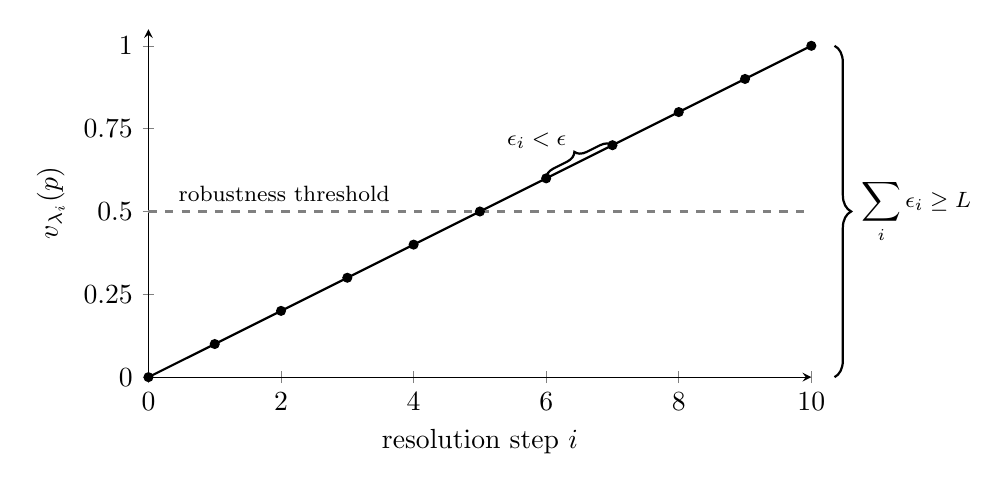
\begin{tikzpicture}
\begin{axis}[
  width=10cm, height=6cm,
  xlabel={resolution step $i$},
  ylabel={$v_{\lambda_i}(p)$},
  xmin=0, xmax=10, ymin=0, ymax=1.05,
  xtick={0,2,...,10},
  ytick={0,0.25,0.5,0.75,1},
  axis lines=left,
  every axis plot/.append style={black},
  clip=false
]
\addplot[mark=*, mark size=1.4pt, thick] coordinates {
(0,0) (1,0.1) (2,0.2) (3,0.3) (4,0.4) (5,0.5) (6,0.6) (7,0.7) (8,0.8) (9,0.9) (10,1.0)
};
\addplot[dashed, gray, thick, domain=0:10] {0.5}
  node[pos=0.03, above, black, font=\footnotesize, anchor=south west] {robustness threshold};
\draw[decorate, decoration={brace, amplitude=4pt}, thick]
  (axis cs:6,0.6) -- (axis cs:7,0.7)
  node[midway, above left=1pt, font=\footnotesize] {$\epsilon_i < \epsilon$};
\draw[decorate, decoration={brace, mirror, amplitude=6pt}, thick]
  (axis cs:10.35,0) -- (axis cs:10.35,1.0)
  node[midway, right=6pt, font=\footnotesize] {$\displaystyle\sum_i \epsilon_i \geq L$};
\end{axis}
\end{tikzpicture}
\caption{Dispersion under refinement. Each increment
$|v_{\lambda_{i+1}}(p) - v_{\lambda_i}(p)| = \epsilon_i$ falls below any
reasonable local threshold $\epsilon$, yet the accumulated displacement
$\sum_i \epsilon_i$ crosses the predicate's robustness threshold (dashed).
Local smallness does not imply global persistence. No step contains a
disagreement, so this failure is invisible to Chapter 21's overlap
comparison --- dispersion and compatibility obstruction are different
mechanisms.}
\label{fig:dispersion}
\end{figure}

\textbf{Why this had to wait for Chapter 14, and couldn't live in Part III or
Part VI.} Compatibility obstruction, as built in Part III and formalized
further in Part VI, is a fact about disagreement between fixed pieces of
local data at one resolution --- it has no notion of \emph{scale} built into it
at all; two patches either agree or they don't, full stop. Dispersion
obstruction needs a family of resolutions, a distance between values at
adjacent resolutions, and a way of accumulating that distance across the
whole family --- precisely the resolution-profile structure Chapter 14
introduced and Parts III and VI never needed, because bare agreement or
disagreement doesn't carry a magnitude the way accumulation requires.
Vagueness, on this account, isn't a fourth kind of nonclassical semantics
standing beside gaps, gluts, and constructive failure, and it also isn't
merely ``compatibility obstruction plus a scale parameter'' --- it's a
genuinely different mathematical mechanism, a third failure mode
distinguishable from the other two by what it actually requires to
detect it:

\[\boxed{\text{compatibility} \neq \text{continuity} \neq \text{persistence}}\]

Compatibility (Part III, Part VI) asks whether fixed local pieces agree.
Continuity, in whatever sense a topology on a space of configurations
might supply, asks which configurations count as \emph{nearby}. Persistence ---
this chapter's actual subject --- asks whether small displacement,
repeatedly accumulated, stays small. A bare topology encodes the second
without automatically supplying the third: nearness alone doesn't hand
you a magnitude of accumulated displacement unless something further
(a metric, a uniformity, a filtration, or the \(\mathcal{P}\) functional
used here) is layered on top of it.

\textbf{What this chapter leaves open.} Whether \(\mathcal{P}[s] \to 0\), defined
via accumulated pairwise distance, is the right formal target isn't
settled here --- the choice of persistence functional is a modeling
decision, not a derivation. Nor does this chapter resolve the further
question of how dispersion obstruction relates to Part VI's geometric
program (Chapter 23's proposed topology on the support-coherence space),
though the three-way non-collapse above gives whoever revises Part VI
last a specific, answerable test rather than an open-ended comparison:
\textbf{does Chapter 23's proposed topology merely encode neighborhoods and
continuity, or does it contain enough additional structure (a metric,
uniformity, or filtration) to measure persistence under refinement?} If
only the former, this chapter and Chapter 23 are not duplicates --- Chapter
23 supplies the qualitative geometry, and dispersion needs the extra
scale structure this chapter has now made explicit on top of it. If the
topology turns out already to contain that structure, that's worth
knowing too, but it should be discovered by testing Chapter 23 against
this question, not assumed either way in advance.

\hypertarget{status-of-this-draft}{%
\section{Status of this draft}\label{status-of-this-draft}}

Revised once already, on substantive rather than stylistic grounds.
Chapter 13's central claim is now pinned to \(\neg\neg p \to p\) failing
specifically, rather than a looser slogan about inferring existence from
absurdity, which was directionally right but risked overstating how
simple intuitionistic negation is. Chapter 14 now explicitly labels
resolution-stability as this book's proposed interpretation of degree,
not something many-valued semantics already meant, and introduces the
resolution profile \(\lambda \mapsto v_\lambda(p)\) as the object that
actually carries the needed structure. Chapter 15's original definition
of dispersion obstruction was mathematically broken --- exact local
agreement cannot produce global disagreement, by transitivity alone ---
and has been replaced with the correct mechanism, accumulated small
variation exceeding a threshold, together with a worked toy example and
the compatibility/continuity/persistence non-collapse. That non-collapse
also converts the earlier open question about Chapter 23 into a specific,
testable one rather than a vague ``are these the same idea'': does Chapter
23's topology contain enough structure to measure persistence, not just
neighborhoods. All three corrections make the chapters more defensible,
not less ambitious --- Chapter 15 in particular went from an evocative
analogy with sorites to an actual mechanism.
